\documentclass[english, 11 pt, class=article, crop=false]{standalone}
\usepackage[T1]{fontenc}
\usepackage[utf8]{luainputenc}
\usepackage{lmodern} % load a font with all the characters
\usepackage{geometry}
\geometry{verbose,a4paper, landscape, inner=2.3cm, outer=1.8 cm, bmargin=1cm, tmargin=1cm}
\setlength{\parindent}{0bp}
\usepackage{import}
\usepackage[subpreambles=false]{standalone}
\usepackage{amsmath}
\usepackage{amssymb}
\usepackage{esint}
\usepackage{babel}
\usepackage{tabu}
\usepackage[dvipsnames, table]{xcolor}
\makeatother
\makeatletter


\begin{document}
\pagestyle{empty}
Skriv dei ufarga tala som eit gongestykke mellom to tall. Skriv inn i boksen under talet. Kalkulator er lov å bruke.
\begin{figure}
	\centering
	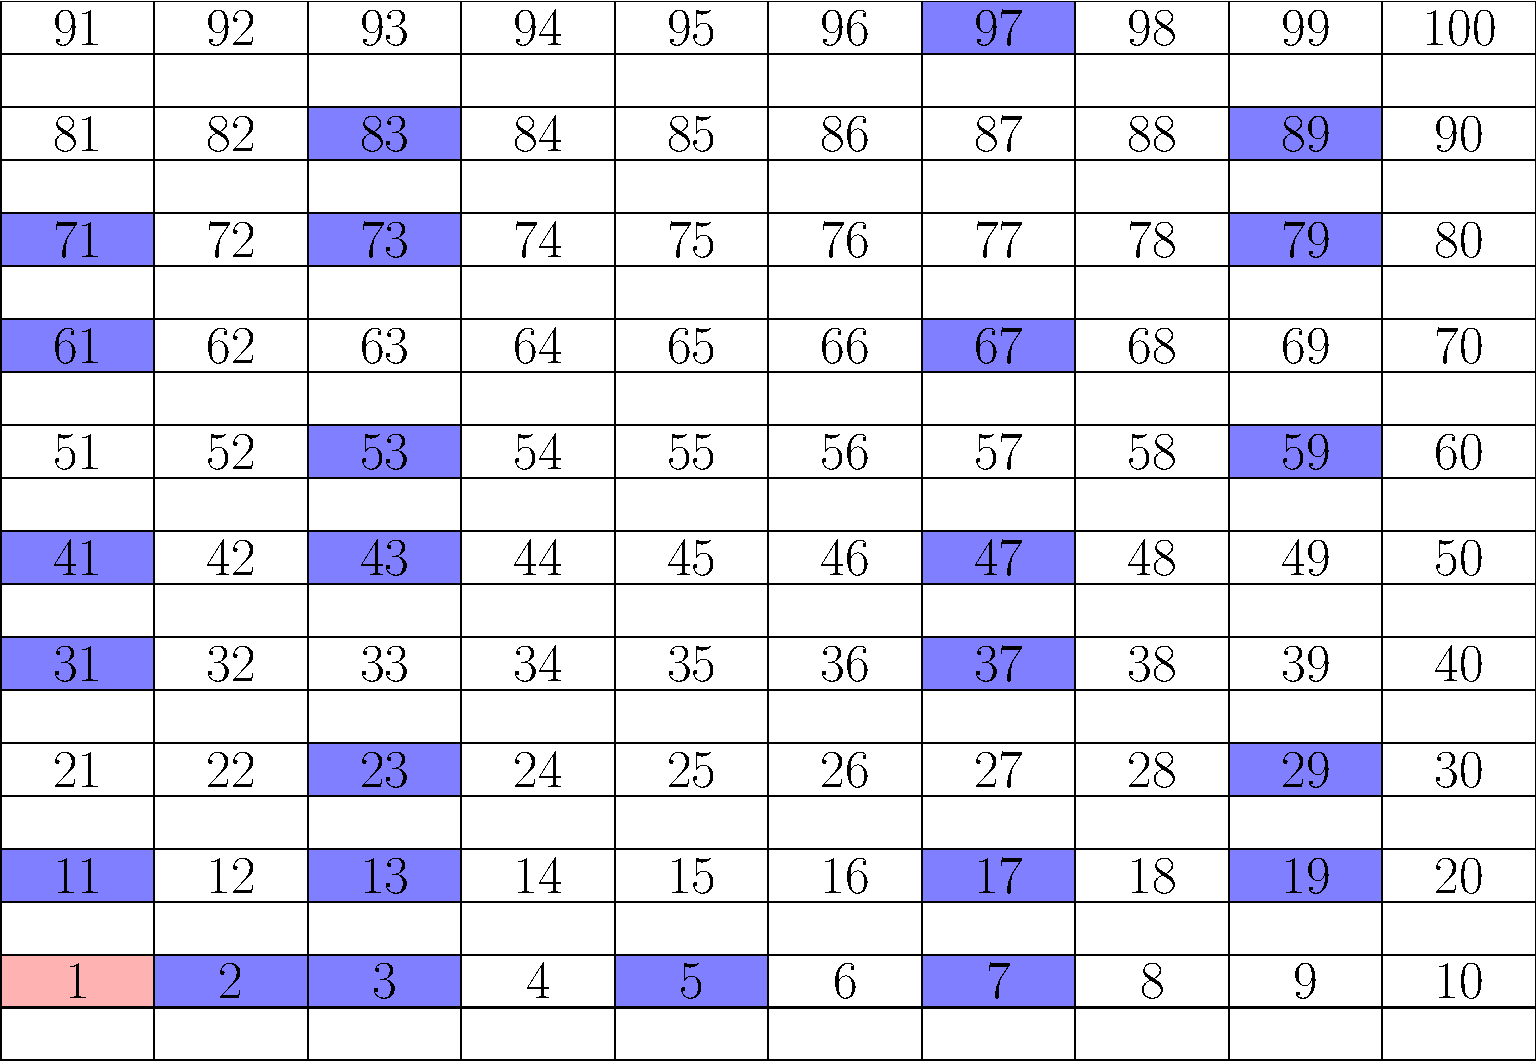
\includegraphics{fakttil100opg}
\end{figure} 
\newpage
\pagestyle{empty}
Primtalsfaktoriser dei ufarga tala. Skriv inn i boksen under talet. Kalkulator er lov å bruke. (Hugs at du kan sjekke svara dine sjølv!)
\begin{figure}
	\centering
	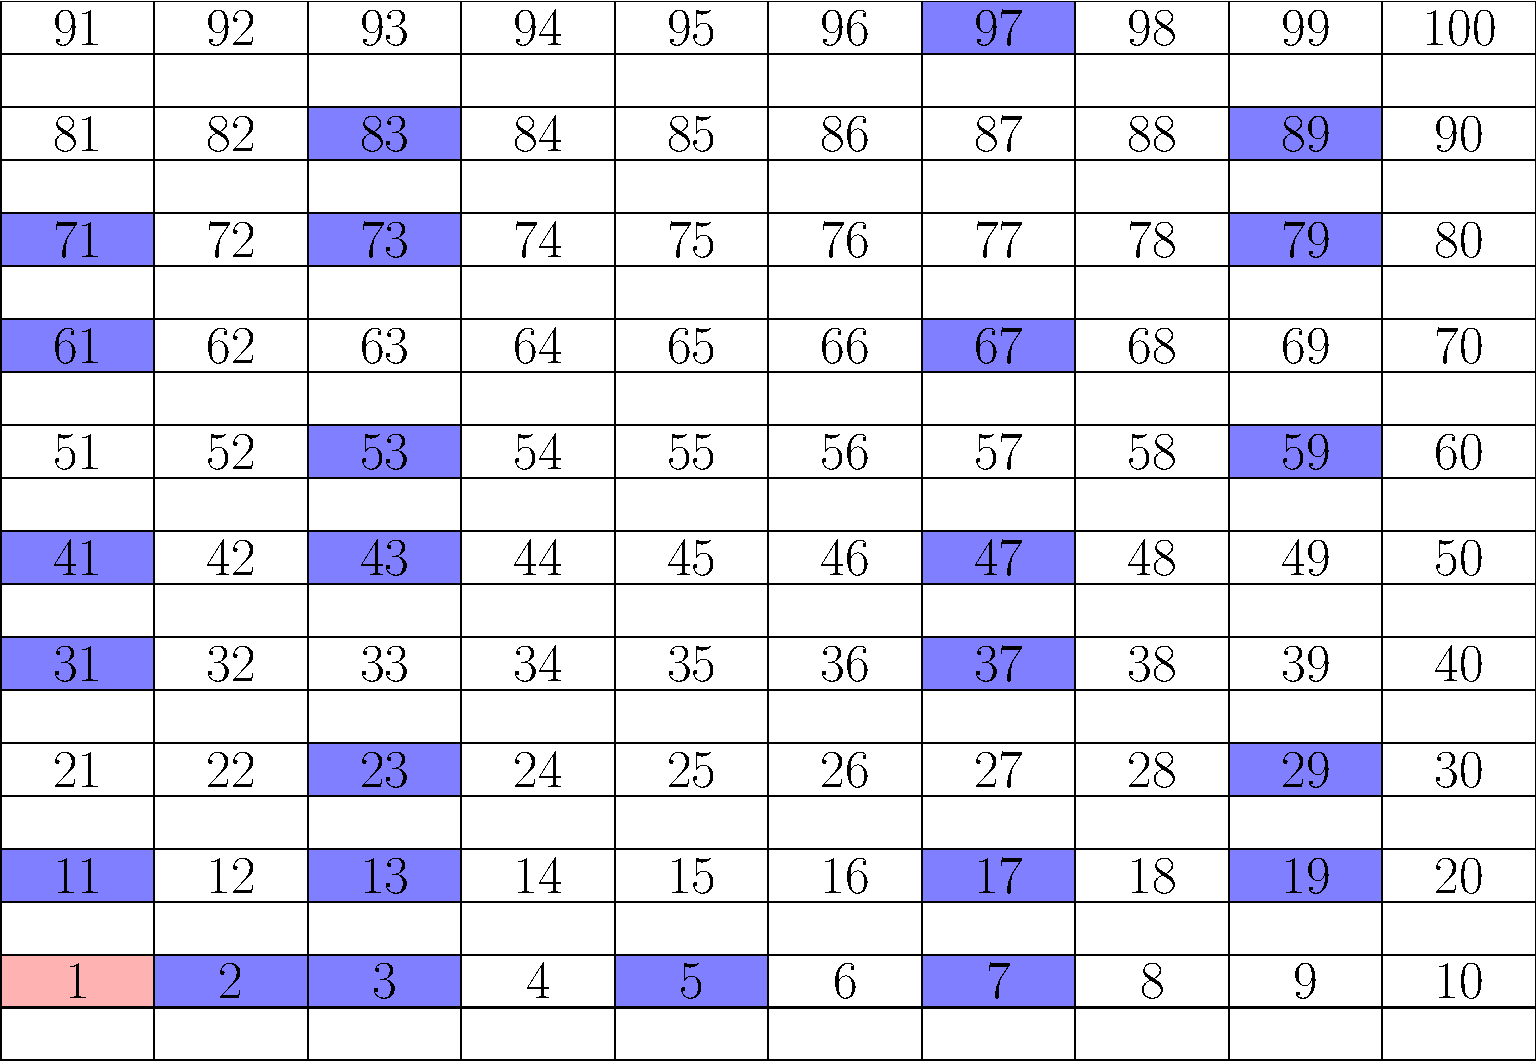
\includegraphics{fakttil100opg}
\end{figure} 

\end{document}